\documentclass[english]{article}

\usepackage{graphicx}
\usepackage{grffile}
\usepackage[T1]{fontenc}
\usepackage{babel}

\author{
	Maree, Armand\\
	\texttt{12017800}
	\and
	Watt, Brenton\\
	\texttt{14032644}
	\and
	Meyers, Charl\\
	\texttt{14024633}
	\and
	Tom, Elton\\
	\texttt{13325095}
	\and
	Tswene, Kamogelo\\
	\texttt{12163555}
	\and
	XXX, Keletso\\
	\texttt{XXXXXXXX}
	\and
	Spazzoli, Lorenzo\\
	\texttt{13304862}
}

\title{Software Requirements Specification\\
	and\\
	Technology Neutral Process Design\\
	\large Name of project\\
	\small Version: 1.0}
\date{\today}

\begin{document}
	\maketitle
	\begin{figure}[!t]
		
\includegraphics[width=\linewidth]{up_logo.png}
	\end{figure}
	\pagenumbering{gobble}
	\newpage
	\tableofcontents
	\newpage
	\pagenumbering{arabic}
	
	\section{Introduction}
		\paragraph\indent
			In this document it would be specified how a system would be developed for the department of computer science at the University of Pretoria in order for them to replace their current, not so efficient Microsoft Office Excel spreadsheet, system with a more concurrent and reliable option.

	\section{Vision}
		\paragraph\indent
		The client requires a system that would allow them to retrieve and submit meta-data about academic papers published by the department of computer science at the University of Pretoria. Certain users would be able to create new papers and the project leader would then be able to control certain properties of the project, like the current progress of the paper. It should also have a web interface where changes can be made and also an Android app.

	\section{Background}
	
	\section{Architecture Requirements}
		\subsection{Access channel requirements}
			\paragraph\indent
			The system requires 2 interfaces:
			\begin{list}{$\bullet$}{\leftmargin=1.5cm \itemindent=0em}
				\item Web interface
				\item Android app
			\end{list}

		\subsection{Quality requirements}
			\paragraph\indent
			The following quality aspects needs to be addressed:
			\begin{list}{$\bullet$}{\leftmargin=1.5cm \itemindent=0em}
				\item \textbf{Scalability:} About a 1000 users will use the system.
				\item \textbf{Security:} Passwords will be hashed with the SHA512 hashing algorithm.
				\item \textbf{Reliability:} An automatic full dump backup will be done everyday at 03:00 and each back up will be kept for a week.
				\item \textbf{Auditability:} Every change should be logged and the person responsable for that log will be recorded. This will allow the administrators to track which users change what.
				\item \textbf{Maintainability:} Data that is deleted will only be moved to another database that might be a little slower. This will help alleviate some pressure off the main database.
				\item \textbf{Cost:} The total hours is estimated to be 120 at a cost of R500 per hour.
			\end{list}
			
		\subsection{Integration requirements}
			\paragraph\indent
			The system should allow universities to connect to each other using an API. This would allow them collaborate on projects and also to track the papers that is being written. The Android app should also be able to connect to the server via the API.
			
			\paragraph\indent
			The protocol that will be used to transfer the data between the server and the clients will be the Hyper Text Transfer Protocol Secure (HTTPS). And the third parties that integrate with the system will access it either through the web interface, the mobile app or the provided API.
			
			\paragraph\indent
			Some quality requirements that has to be considered are:
			\begin{list}{$\bullet$}{\leftmargin=1.5cm \itemindent=0em}
				\item \textbf{Security:} The data that is sent over the internet should be encrypted and it has been decided to use the Secure Socket Layer (SSL) encryption algorithm.
				\item \textbf{Reliability:} The reliability of the transfer of the data is dependant on the reliability of the internet connection.
			\end{list}
		\subsection{Architecture constraints}
			\paragraph\indent
			There are currently no architecture constraints that the client mentioned.
			

	\section{Functional requirements and application design}
		\subsection{Use case prioritization}
		\paragraph\indent
		\textbf{Critical:}
			\begin{list}{$\bullet$}{\leftmargin=1.5cm \itemindent=0em}
				\item There must be some web hosting server in order to be able to host a web interface, this interface will be the main 
				access chanel to the system as it makes it easier ti access the system on a computer or non-Android device. If there is no webserver then there will be no web interface that can be accessed from research groups all over the country. This defeats the whole purpose of the system.
				\item The web interface needs to be accessible from the Internet preferably so that other research groups outside the University are able to access the system.
				\item The system needs to be able to save data in some way. If there is no possible way to store data then the system might as well not exist, because the purpose of the sysem is to store metadata about research papers.							
			\end{list}
		\paragraph\indent
		\textbf{Important:}
		\begin{list}{$\bullet$}{\leftmargin=1.5cm \itemindent=0em}				
			\item Users must be able to download a bibliography of papers released in a selected period.
			\item An Android app must be available that can access the system to make it easier to access the system on the go.			
			\item Users must create their user profile manually and will not be able to link the system with a web service in order to create their profile.
			\item No item should ever be deleted in the system. Evrything is kept. Old unaccessed data may be archived but never deleted. There needs to be some sort of recovery or backup system that enables a user to restore accidently deleted data.
			\item The system must be able to handle a max of at least 50 concurrent users as there is a possiblility that at least 50 users may access the system all at once. There will also be an estimate of at least a 1000 users. The system must be able to handle that amount of users.
		\end{list}
		\paragraph\indent
		\textbf{Nice-to-have:}
		\begin{list}{$\bullet$}{\leftmargin=1.5cm \itemindent=0em}
			\item The system must be lightweight.
			\item The system must show a the completion of a paper in percentage that a user specifies after editing the paper.
			\item The system may link with Google Calender to synchronise due dates and alerts for the paper a user is busy working on.
			\item The web interface can be designed to work on mobile phones for those who want to access the system on the go but do not have an Android device.
		\end{list}
		
		\subsection{Use case/Services contracts}
			\paragraph\indent
			\textbf{Pre-Conditions:}
				\begin{list}{$\bullet$}{\leftmargin=1.5cm \itemindent=0em}
					\item Only the author(s) of a paper can edit the paper, unless a non-author has been assigned the right to do so.
					\item Only the authur(s) can view details about the paper, unless a the non-author has been assigned the right to do so.
					\item Non-users are not authorized to view a paper.
				\end{list}
			\paragraph\indent
			\textbf{Post-Conditions:}
				\begin{list}{$\bullet$}{\leftmargin=1.5cm \itemindent=0em}
					\item Once an author as been assigned to a paper they have to remain as an author of that paper in order to continue viewing and editing it.
					\item Once a user has closed their account they will lose access to the papers they had access to.
				\end{list}
			\paragraph\indent
			\textbf{Request and Results Data Structures:}
				\begin{figure}[!h]
					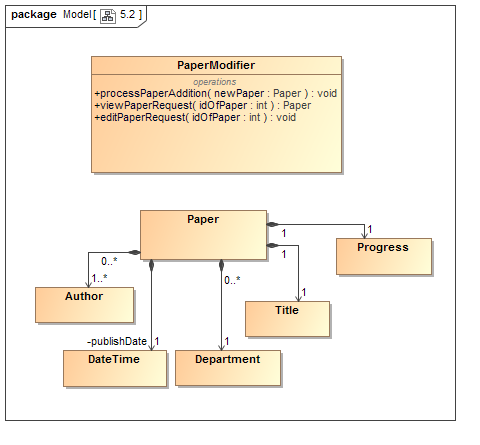
\includegraphics[width=\linewidth]{5.2.png}
				\end{figure}

		\subsection{Required functionality}

		\subsection{Process specifications}

		\subsection{Domain Model}

	\section{Open Issues}
		\begin{list}{$\bullet$}{\leftmargin=1.5cm \itemindent=0em}
			\item Item 1
			\item Item 2
		\end{list}
\end{document}
